\documentclass[11pt,a4paper]{article}

\usepackage[margin=1in]{geometry}
\usepackage{graphicx}
\usepackage{float}
\usepackage{hyperref}
\usepackage{xcolor}
\usepackage{listings}
\usepackage{booktabs}
\usepackage{array}
\usepackage{setspace}

\hypersetup{
  colorlinks=true,
  linkcolor=blue,
  urlcolor=blue
}

\lstdefinestyle{labcode}{
  basicstyle=\ttfamily\small,
  breaklines=true,
  frame=single,
  numbers=left,
  numberstyle=\tiny,
  keywordstyle=\color{blue},
  commentstyle=\color{teal},
  stringstyle=\color{orange!80!black},
  showstringspaces=false
}

\title{Intelligent Robots Lab 6 Report\\Zaoer Bot Gazebo Simulation}
\author{Prepared for submission to Blackboard}
\date{\today}

\begin{document}
\maketitle
\onehalfspacing

\section{Task Overview}
The goal of Lab 6 is to create a robot model of ``myself'', add a camera and a lidar sensor, load the robot into Gazebo, complete sensor simulation, and display the sensor data in RViz. The final submission also needs to include the catkin packages and a report with code, running steps, results, and analysis.

To satisfy the task, I designed a self-inspired differential-drive robot named \texttt{zaoer\_bot}. The robot uses a stylized upper-body appearance mounted on a mobile base, and includes:

\begin{itemize}
  \item a monocular front camera publishing \texttt{/camera/image\_raw} and \texttt{/camera/camera\_info},
  \item a 2D lidar publishing \texttt{/scan},
  \item a Gazebo world with obstacles so the sensors produce visible output,
  \item an RViz configuration for visualizing the robot and the sensor data.
\end{itemize}

\section{Package Structure}
The submission contains two catkin packages.

\begin{center}
\begin{tabular}{>{\ttfamily}p{0.35\linewidth} p{0.55\linewidth}}
\toprule
Package / File & Purpose \\
\midrule
zaoer\_bot\_description & Robot Xacro/URDF model \\
zaoer\_bot\_gazebo & Gazebo world, launch files, RViz config, capture script \\
urdf/zaoer\_bot.urdf.xacro & Main robot body, wheels, camera, lidar, Gazebo plugins \\
launch/view\_zaoer\_bot\_lab\_world.launch & Start Gazebo world and spawn robot \\
rviz/zaoer\_bot\_sensors.rviz & RViz visualization configuration \\
scripts/capture\_lab6\_results.sh & Automated screenshot and topic capture \\
\bottomrule
\end{tabular}
\end{center}

\section{Robot Design}
\subsection{Mechanical Model}
The robot is based on a differential-drive chassis because it is stable and easy to simulate. To reflect the ``robot model of yourself'' requirement, the body includes a torso, head, arms, chest badge, and backpack-style rear body using primitive shapes. Primitive geometry keeps the package lightweight and easy to compile.

The main physical structure is:

\begin{itemize}
  \item \texttt{base\_link}: torso and decorative visuals,
  \item \texttt{left\_wheel\_link}, \texttt{right\_wheel\_link}: drive wheels,
  \item \texttt{rear\_caster\_link}: rear support,
  \item \texttt{camera\_link}: front-facing camera on the head,
  \item \texttt{lidar\_link}: 2D lidar on the top of the head.
\end{itemize}

\subsection{Sensors}
Two sensor models were added in Gazebo:

\begin{itemize}
  \item Camera sensor with \texttt{libgazebo\_ros\_camera.so}
  \item Ray-based lidar sensor with \texttt{libgazebo\_ros\_laser.so}
\end{itemize}

The key camera configuration is shown below.

\begin{lstlisting}[style=labcode,language=XML]
<gazebo reference="camera_link">
  <sensor type="camera" name="front_camera_sensor">
    <always_on>true</always_on>
    <update_rate>20.0</update_rate>
    <camera name="front_camera">
      <horizontal_fov>1.047</horizontal_fov>
      <image>
        <width>640</width>
        <height>480</height>
        <format>R8G8B8</format>
      </image>
    </camera>
    <plugin name="zaoer_camera_controller"
            filename="libgazebo_ros_camera.so">
      <cameraName>camera</cameraName>
      <imageTopicName>image_raw</imageTopicName>
      <cameraInfoTopicName>camera_info</cameraInfoTopicName>
      <frameName>camera_optical_frame</frameName>
    </plugin>
  </sensor>
</gazebo>
\end{lstlisting}

The lidar configuration is:

\begin{lstlisting}[style=labcode,language=XML]
<gazebo reference="lidar_link">
  <sensor type="ray" name="lidar_sensor">
    <visualize>true</visualize>
    <update_rate>15.0</update_rate>
    <ray>
      <scan>
        <horizontal>
          <samples>720</samples>
          <min_angle>-1.5708</min_angle>
          <max_angle>1.5708</max_angle>
        </horizontal>
      </scan>
      <range>
        <min>0.12</min>
        <max>8.0</max>
      </range>
    </ray>
    <plugin name="zaoer_lidar_controller"
            filename="libgazebo_ros_laser.so">
      <topicName>scan</topicName>
      <frameName>lidar_link</frameName>
    </plugin>
  </sensor>
</gazebo>
\end{lstlisting}

\subsection{Motion Model}
The robot uses the Gazebo differential drive plugin so the mobile base publishes odometry and wheel joint states while listening to \texttt{/cmd\_vel}.

\begin{lstlisting}[style=labcode,language=XML]
<gazebo>
  <plugin name="zaoer_diff_drive" filename="libgazebo_ros_diff_drive.so">
    <leftJoint>left_wheel_joint</leftJoint>
    <rightJoint>right_wheel_joint</rightJoint>
    <wheelSeparation>0.38</wheelSeparation>
    <wheelDiameter>0.12</wheelDiameter>
    <commandTopic>cmd_vel</commandTopic>
    <odometryTopic>odom</odometryTopic>
    <robotBaseFrame>base_footprint</robotBaseFrame>
  </plugin>
</gazebo>
\end{lstlisting}

\section{Simulation Environment}
To make the sensor output meaningful, I created a simple obstacle world instead of using a completely empty world. The world contains:

\begin{itemize}
  \item four boundary walls,
  \item one orange box,
  \item one green cylinder,
  \item one purple panel.
\end{itemize}

These objects are placed in front of and around the robot so both the camera and the lidar can observe them.

\section{Running Steps}
\subsection{Build}
\begin{lstlisting}[style=labcode,language=bash]
cd ~/catkin_ws/src
cp -r zaoer_bot_description zaoer_bot_gazebo .
cd ~/catkin_ws
catkin_make
source devel/setup.bash
\end{lstlisting}

\subsection{Launch The Robot In Gazebo}
\begin{lstlisting}[style=labcode,language=bash]
roslaunch zaoer_bot_gazebo view_zaoer_bot_lab_world.launch
\end{lstlisting}

\subsection{Optional Automatic Capture}
\begin{lstlisting}[style=labcode,language=bash]
bash src/zaoer_bot_gazebo/scripts/capture_lab6_results.sh ~/lab6_capture
\end{lstlisting}

\section{Running Results}
\subsection{Gazebo Result}
Figure~\ref{fig:gazebo} shows the robot successfully spawned in the obstacle world.

\begin{figure}[H]
  \centering
  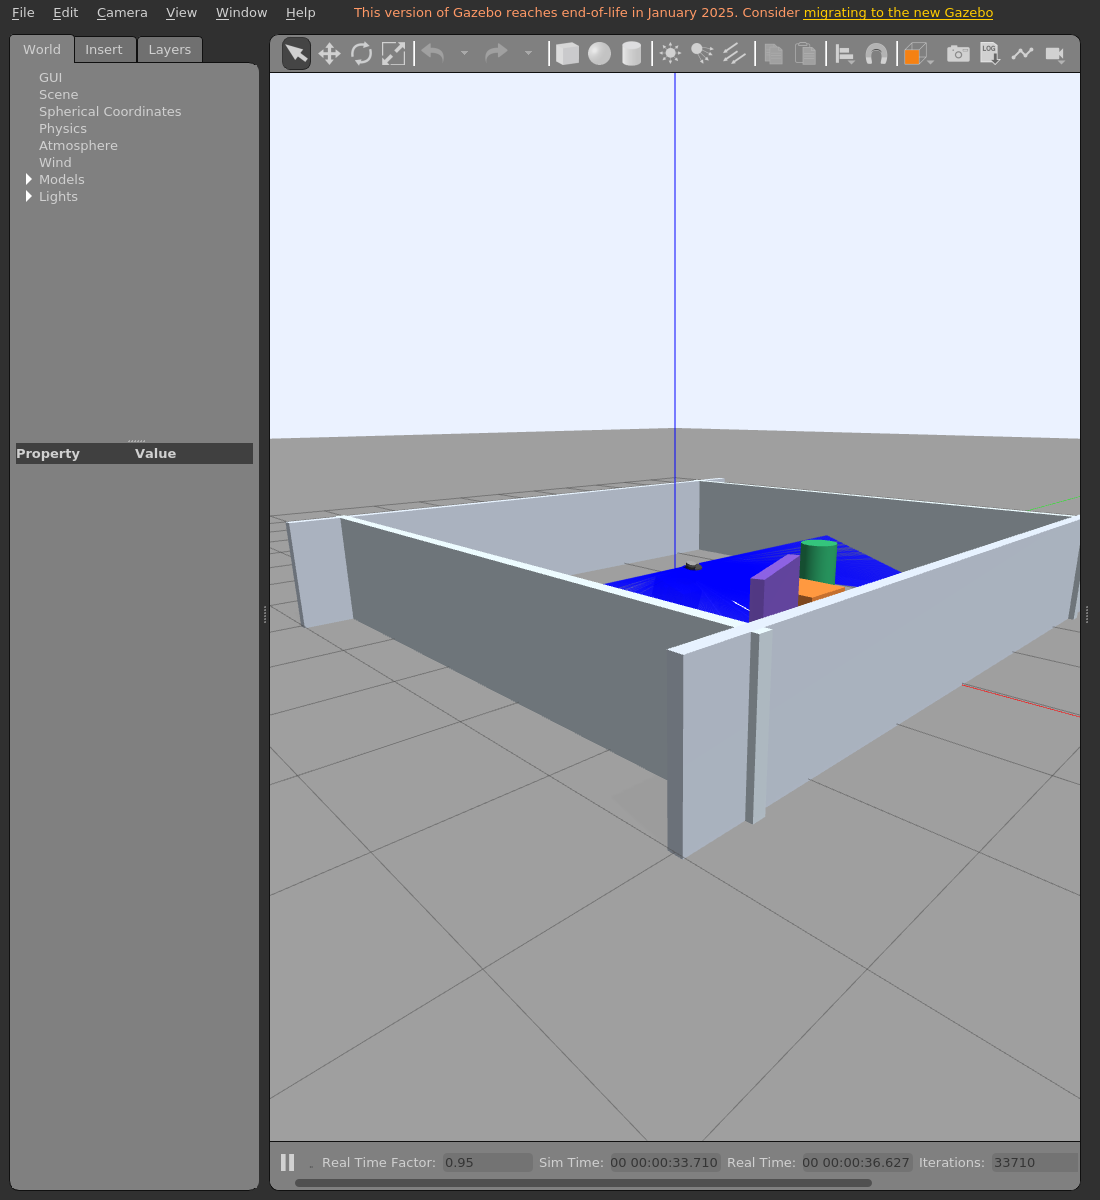
\includegraphics[width=0.72\linewidth]{images/gazebo.png}
  \caption{Gazebo simulation result}
  \label{fig:gazebo}
\end{figure}

\subsection{RViz Result}
Figure~\ref{fig:rviz} shows the RViz visualization. The upper render panel uses the camera display, while the lidar scan is overlaid as red points/lines. This confirms that the sensor data is being published and visualized in RViz.

\begin{figure}[H]
  \centering
  
\includegraphics[width=0.85\linewidth]{images/rviz.png}
  \caption{RViz result with sensor visualization}
  \label{fig:rviz}
\end{figure}

Figure~\ref{fig:desktop} shows Gazebo and RViz running together in the same session.

\begin{figure}[H]
  \centering
  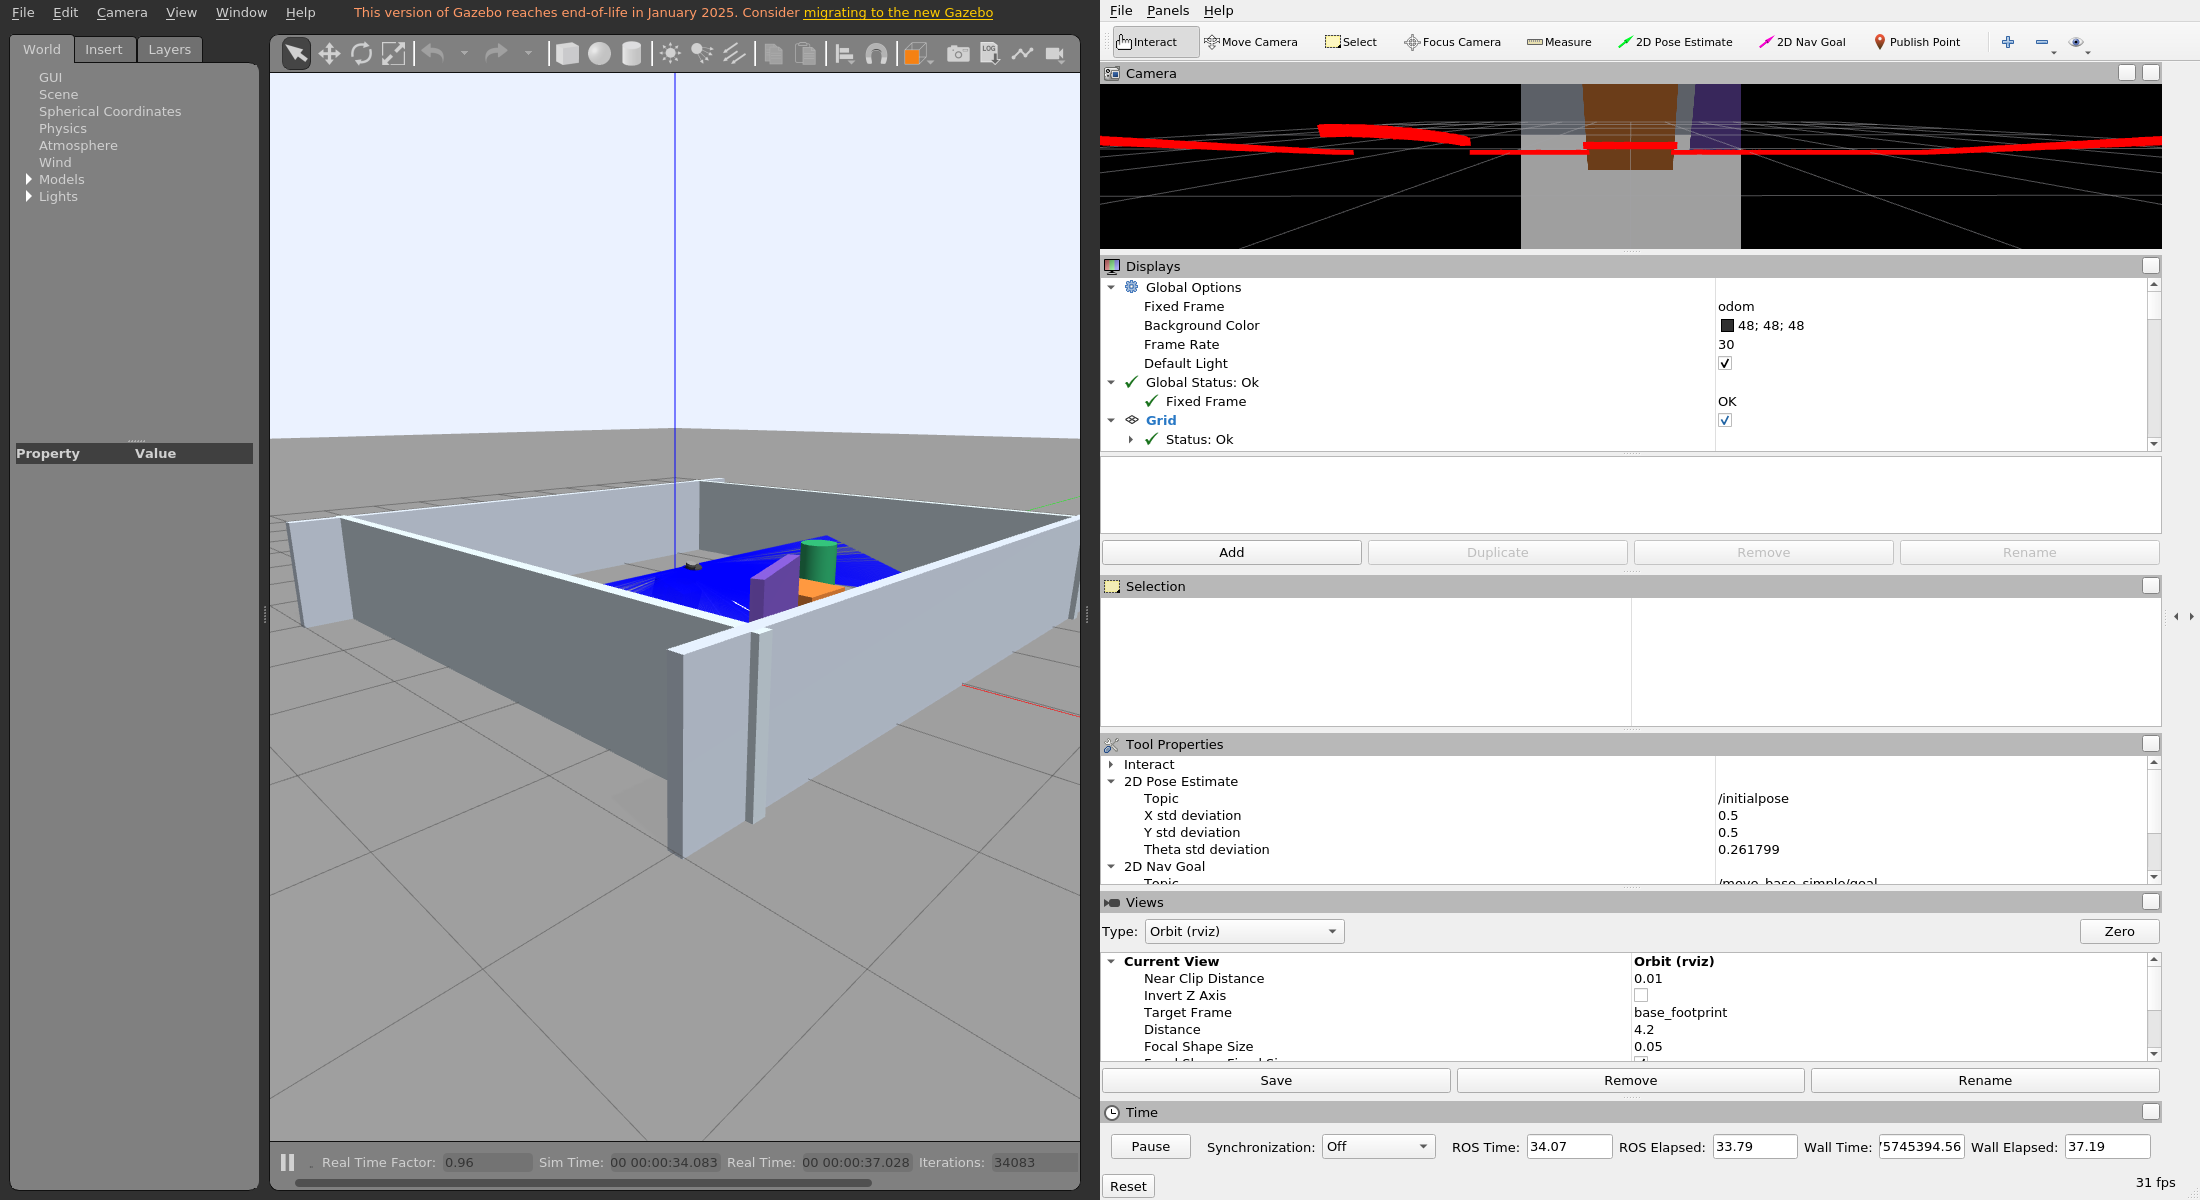
\includegraphics[width=\linewidth]{images/desktop.png}
  \caption{Combined Gazebo and RViz desktop capture}
  \label{fig:desktop}
\end{figure}

\subsection{Published Topics}
The main topics captured during the experiment are:

\begin{lstlisting}[style=labcode]
/camera/camera_info
/camera/image_raw
/clock
/cmd_vel
/joint_states
/odom
/scan
/tf
/tf_static
\end{lstlisting}

The lidar sample shows valid distance data, and the camera information topic was also published correctly.

\section{Result Analysis}
\begin{itemize}
  \item The lidar simulation worked immediately in both headless and GUI modes, publishing valid \texttt{/scan} data.
  \item The camera plugin required a rendering context. In practice, the camera topics appeared correctly when Gazebo was launched with GUI support inside \texttt{Xvfb}. This is why the final capture script uses \texttt{Xvfb} and \texttt{gui:=true}.
  \item The RViz configuration successfully visualized sensor data. The camera panel and overlaid scan confirm that the robot can perceive the surrounding obstacles.
  \item The self-inspired robot model is lightweight because it uses boxes, cylinders, and spheres instead of external meshes. This makes the project portable and easy to rebuild on another ROS Noetic machine.
\end{itemize}

\section{Conclusion}
This Lab 6 submission completes all required parts:

\begin{itemize}
  \item a self-inspired robot model was created,
  \item a camera and a lidar were added,
  \item the robot was loaded into Gazebo,
  \item the sensor simulation was completed,
  \item the sensor data was displayed in RViz,
  \item catkin packages and a report were prepared for submission.
\end{itemize}

The final submission folder includes the source packages, launch files, world file, RViz configuration, capture script, screenshots, and this report.

\end{document}
